\documentclass[12pt]{article}

\linespread{1}

\makeatletter
% ADDS SECTION `S''s
\renewcommand*{\p@section}{\S\,}
\renewcommand*{\p@subsection}{\S\,}
\renewcommand*{\p@subsubsection}{\S\,}
\makeatother

%PACKAGES
\usepackage[T1]{fontenc}
\usepackage[english]{babel}
\usepackage{color}
\usepackage{enumerate}
\usepackage[textheight = 680pt]{geometry}
\usepackage{fancyhdr}
\usepackage{titlesec}
\usepackage{float}
\usepackage[T1]{fontenc}
\usepackage{fullpage}
\usepackage{graphicx}
\usepackage{hyperref} \hypersetup{colorlinks=true, urlcolor=blue}
\usepackage{menukeys}
\usepackage{ifpdf}
\usepackage{listings}
\usepackage{yfonts}

% STYLE FOR USING MDFRAMED PACKAGE
\usepackage{mdframed}

\mdfdefinestyle{MyFrame}{%
    linecolor=red,
    outerlinewidth=10pt,
    roundcorner=20pt,
    innertopmargin=\baselineskip,
    innerbottommargin=\baselineskip,
    innerrightmargin=20pt,
    innerleftmargin=20pt,
    backgroundcolor=gray!10!white}
    
\mdfdefinestyle{CommandFrame}{%
    linecolor=black,
    outerlinewidth=10pt,
    roundcorner=20pt,
    innertopmargin=\baselineskip,
    innerbottommargin=\baselineskip,
    innerrightmargin=20pt,
    innerleftmargin=20pt,
    backgroundcolor=white!90!yellow}

\usepackage{tikz}
 
% IN CASE OF WANTING TO ADD CODE
\definecolor{codegreen}{rgb}{0,0.6,0}
\definecolor{codegray}{rgb}{0.5,0.5,0.5}
\definecolor{codepurple}{rgb}{0.58,0,0.82}
\definecolor{backcolour}{rgb}{0.95,0.95,0.92}
 
\lstdefinestyle{mystyle}{
    backgroundcolor=\color{backcolour},   
    commentstyle=\color{codegreen},
    keywordstyle=\color{magenta},
    numberstyle=\tiny\color{codegray},
    stringstyle=\color{codepurple},
    basicstyle=\footnotesize,
    breakatwhitespace=false,         
    breaklines=true,                 
    captionpos=b,                    
    keepspaces=true,                 
    numbers=left,                    
    numbersep=5pt,                  
    showspaces=false,                
    showstringspaces=false,
    showtabs=false,                  
    tabsize=2
}

 
\lstset{style=mystyle}

% ADDING FANCY DIRECTORY PATHS
\newcommand\setnewpathsep[1]
{%
    \tw@declare@style@simple*{paths}{%
       {\ttfamily\CurrentMenuElement}%
    }[%
       #1%
    ]{blacknwhite}
}

% --- reset the path separator (macro expands to original style def) ---
\newcommand\resetpathsep
{%
     \tw@declare@style@simple*{paths}{%
       {\ttfamily\CurrentMenuElement}%
    }[%
       \hspace{0.2em plus 0.1em}%
       \raisebox{0.08ex}{%
          \tikz{\fill[\usemenucolor{txt}] (0,0) -- (0.5ex,0.5ex)%
                    -- (0,1ex) -- cycle;}%
    }%
       \hspace{0.2em plus 0.1em}%
    ]{blacknwhite}
}

\newcommand{\subsubsubsection}[1]{\paragraph{#1}\mbox{}\\}
\setcounter{secnumdepth}{4}
\setcounter{tocdepth}{4}

\pagestyle{fancy}
\setlength{\headheight}{15pt}
\setlength{\headsep}{10pt}
\lhead{M.B. Adams *}
\chead{\emph{University of Rochester}}
\rhead{Head TA Duties}
\lfoot{* e-mail: \href{mailto:madams@pas.rochester.edu}{madams@pas.rochester.edu} }
\title{PHY12$X$P Head Teaching Assistant Duties}
\author{Marissa B. Adams}
\date{\today}

%%%%%%%%%%%%%%%%%%%%%%%%%%%%%%%%%%%%%%%%%%%%%%%%%%%%%%%%%%%
%%%% BEGINNING DOCUMENT %%%%%%%%%%%%%%%%%%%%%%%%%%%%%%%%%%%
%%%%%%%%%%%%%%%%%%%%%%%%%%%%%%%%%%%%%%%%%%%%%%%%%%%%%%%%%%%

\begin{document}

\maketitle
\newpage
\tableofcontents
\newpage

\thispagestyle{fancy}

%%%%%%%%%%%%%%%%%%%%%%%%%%%%%%%%%%%%%%%%%%%%%%%%%%%%%%%%%%%
%%%% INTRODUCTION %%%%%%%%%%%%%%%%%%%%%%%%%%%%%%%%%%%%%%%%%
%%%%%%%%%%%%%%%%%%%%%%%%%%%%%%%%%%%%%%%%%%%%%%%%%%%%%%%%%%%
\section{Introduction}
%%%%%%%%%%%%%%%%%%%%%%%%%%%%%%%%%%%%%%%%%%%%%%%%%%%%%%%%%%%

\indent If you are reading this document perhaps you have been selected to manage and run the Mastery/Self-Paced (MSP) Physics courses at the University of Rochester. There are generally two courses that fit this format: 

\begin{itemize}
	\item PHY122P (\emph{Electricity and Magnetism for Scientists and Engineers}), 
	\item and PHY121P (\emph{Mechanics for Scientists and Engineers}). 
\end{itemize}

\noindent Hence the generality of PHY12$X$P ($X=1,2$) to indicate that these materials can be used for either course. The former generally takes place during the Fall semesters, and the latter, the Spring. Both courses are freshman-sophomore level physics courses that are generally aimed at engineering students. Both courses follow the framework under the MSP philosophy. 

\indent One stark difference is that PHY122P has 12 modules, while PHY121P has 13. The number of modules is tried and true, however there is much room for course development, and statistical analysis in a MSP course. It is up to the professor to decide if they would like to make some changes during before the semester begins. This document will detail the general flow for such a course through all 12-13 modules, perhaps some of the history of MSP courses at the University of Rochester, and general Head TA guidelines that will make the role manageable to even someone new to MSP. The document may be long and perhaps intimidating, but all of the information is there to help someone who just stepped into the department the day before they are reading this. 

\newpage
%%%%%%%%%%%%%%%%%%%%%%%%%%%%%%%%%%%%%%%%%%%%%%%%%%%%%%%%%%%
%%%% COURSE FLOW %%%%%%%%%%%%%%%%%%%%%%%%%%%%%%%%%%%%%%%%%%
%%%%%%%%%%%%%%%%%%%%%%%%%%%%%%%%%%%%%%%%%%%%%%%%%%%%%%%%%%%
\section{Course Flow} \label{sec:cf}
%%%%%%%%%%%%%%%%%%%%%%%%%%%%%%%%%%%%%%%%%%%%%%%%%%%%%%%%%%%

Here we generally describe the tasks needed at certain parts of the course. In the beginning of the course we generally mean before the course begins, and within the first month of the course. The middle of the course generally consists of the 2-3 months within the middle of the semester. The end of the course is clearly the last month of the course, including the finals week. You can probably see from these lists that the majority of the responsibility goes into setting up the course. Generally the pace of the course for the head TA for the majority of the semester is pretty relaxed outside of teaching in the workshop.

%%%%%%%%%%%%%%%%%%%%%%%%%%%%%%%%%%%%%%%%%%%%%%%%%%%%%%%%%%%
\subsection{Course Beginning} \label{sec:cb}

\begin{itemize}
	\item Understand how the scripts and processing tools work, and what is required of you throughout the semester. Reading this document is a good start, and playing around with the git-repo (\ref{sec:gitrepo}).
	\item Draft a TA/TI schedule (\ref{sec:schedule}).
	\item Create the google document that is the quiz schedule (\ref{sec:qs}).
	\item Work with the professor to set up the courses blackboard and populate it with the information both students and your staff will need to run the course. You may actually get students who do the module workshops before the semester begins and finish before the end of the first month (\ref{sec:gc}).
	\item Right before the beginning of the semester, start implementing the TA/TI training, and ensure that your staff feels comfortable with what is required of them (\ref{sec:training}).
	\item Around this time the professor is probably working on the syllabus and a presentation to give to the class about the course structure, you can expect to be apart of that process.
	\item You'll want to send a welcome e-mail to the class that includes a lot of these things you've been creating for the course (schedules, information, how to access things on Blackboard, contact information, etc).
	\item Once the semester begins you will want to be involved in the workshops to make sure that everything is running smoothly.
	\item Be aware that during this time students typically add/drop the course.
	\item Many iterations to the TA/TI schedule may happen during this time. You may need to ask for more staff members from the professor who assigns TA/TI roles.
	\item Start running the scripts after the first week and start sending out weekly e-mails!
	\item Note that you will probably see a lot of empty spaces in the quiz schedule at this time.
\end{itemize}

%%%%%%%%%%%%%%%%%%%%%%%%%%%%%%%%%%%%%%%%%%%%%%%%%%%%%%%%%%%
\subsection{Course Middle} \label{sec:cm}

\begin{itemize}
	\item At this point you will want to be running your scripts and checking the progress (\ref{sec:ocp} and pass rates (\ref{sec:cpr}) for the course.
	\item Students who are lagging behind you will want to forward information about over to Nick Valentino, or whomever is running the efforts at the Hajim School to keep track of behind students. 
\end{itemize}

%%%%%%%%%%%%%%%%%%%%%%%%%%%%%%%%%%%%%%%%%%%%%%%%%%%%%%%%%%%
\subsection{Course End} \label{sec:ce}

\begin{itemize}
	\item Keep on with the scripts and processing until the very last workshop.
	\item Do not allow for ``Grade-a-thons.'' Students may ask for more quiz slots as time starts running out. The quiz slots will probably be all taken up by the last week.
	\item Coordinate with the lecture based course on how the final will be graded.
\end{itemize}


%%%%%%%%%%%%%%%%%%%%%%%%%%%%%%%%%%%%%%%%%%%%%%%%%%%%%%%%%%%
%%%% DUTIES %%%%%%%%%%%%%%%%%%%%%%%%%%%%%%%%%%%%%%%%%%%%%%%
%%%%%%%%%%%%%%%%%%%%%%%%%%%%%%%%%%%%%%%%%%%%%%%%%%%%%%%%%%%
\section{Duties} \label{sec:duties}
%%%%%%%%%%%%%%%%%%%%%%%%%%%%%%%%%%%%%%%%%%%%%%%%%%%%%%%%%%%

\indent Here we detail duties that typically the Head Teaching Assistant would carry out before, and during the semester they are teaching. You can find a general outline for when these duties are typically carried out in \ref{sec:cf}.

%%%%%%%%%%%%%%%%%%%%%%%%%%%%%%%%%%%%%%%%%%%%%%%%%%%%%%%%%%%
\subsection{TA/TI Training} \label{sec:training}

\indent You will be informed of if you're the Head TA by either the professor in charge of the course, or the professor in charge of designating the TA/I positions. This role is typically played by Professor Steven Teitel. Once you have been informed of your role, typically you also will be given a list of names and e-mails for the rest of the folks on the MSP staff. At this point it is up to you and the professor in charge of the course to come up with a suite of dates to propose to the staff of when to hold the TA/I training.

\indent Before the beginning of the semester there is generally a ``prime'' period to conduct the Teaching Assistant and Instructor Training. For the Fall semesters the first week or days before classes begin folks have already arrived back in Rochester (if they have left). Similarly for the Spring semester. One may want to be wary for second and third year students however, who may need to teach again and simultaneously take the preliminary exam, which is typically at the end of August. The department holds its own TA/I training that it requires all of its graduate students to go through, and potentially undergraduates if they are enrolled as a teaching instructor. 

\indent Due to the unique nature of MSP, we find it beneficial to hold our own TA/I training to go over the philosophy of the course, get to know the team and build camaraderie, specific duties one can play in the workshop, and which ones are typically filled by graduate students and undergraduates. Typically the meeting is held in the room where the MSP course takes place, Bausch and Lomb Hall 208. One can find TA/I training materials to pass out to the staff, and also familiarize yourself with, in the \texttt{git} repo (\ref{sec:gitrepo}). There are some intricacies, such as how to utilize the grade center in blackboard as prescreener versus a grader that are necessary to go over before the course begins.

\vspace{10pt}

\noindent \textbf{Checklist you may want to follow through on for scheduling the training/before the training:}

\begin{itemize}
	\item Once you've gotten the contact info for the staff and have met with the professor running the course, draft and e-mail that includes a doodle poll (\url{http://doodle.com/}, or whatever scheduling application you prefer to use) for the TA/I training with a range of dates and types. You can expect that some people cannot make any of these times\footnote{Generally for these folks it would be easiest once you have the TA/I schedule made to assist them on their first workshop to answer questions they have and make sure they are following through on the process. Extra training meetings aren't necessary to schedule.}.
	\item In this e-mail you can even introduce yourself a bit. 
	\item Include attached PDFs of the grader, prescreener and workshop leader ``instructions'' or guidelines in the e-mail. There is also another cohesive document in the \texttt{git} repo that includes more information.
	\item Also query the staff for screenshots of their schedule, and times that they could not be at the workshop, to help you make a mock up TA/I schedule so that you can go over it in the meeting\footnote{Do not expect for this to be the first and last schedule you make -- there will be iterations.}.
	\item Print out the documents you've sent the staff if you think it'll be necessary at the meeting.
	\item You can ask the under/graduate coordinator, or the professor of the course to print out photos of the students. You may want to give these to each individual staff member as it may help them with names.
	\item Secure the lockers near the entrances to the tunnels of B\& L. Typically you can get the codes and everything figured out with the help of the undergraduate coordinator. 
	\item Keys to B\& L 208: 1 set for the professor, 1 set for you, and two sets on lanyards to put in the lockers near the tunnel entrance of B\& L.
\end{itemize}

\noindent \textbf{Checklist of items to go over during the training:}

\begin{itemize}
	\item Get to know everyone. Do a corny ice-breaker. Make sure you take away people's names, and affiliations, etc.
	\item Ask everyone for their gmail account, in order to give access to the quiz schedule (so they can edit).
	\item Go over the roles:
		\begin{itemize}
			\item Graduate students are required to work 16 hours. They are required to take on more workshops; typically 4-5.
			\item Undergraduate students are required to work 8 hours\footnote{This can vary based on how many credit or pay they have agreed on. You'll be informed of someone's situation by the time the meeting is over.} so they typically sign up for 2 workshops.
			\item Go over the role of prescreener, workshop leader, and grader. Typically we aim to have all three of these roles operating each workshop, so encourage folks to transition between all three. However you'll notice as the semester goes on, some folks stick to one thing.
		\end{itemize}
	\item Ensure that everyone is familiar with how to input having (i) prescreened, (ii) scheduled, (iii) given a quiz, and finally (iv) their pass/fail on the quiz in the blackboard system.
	\item Show the staff the process of scheduling a quiz in the quiz schedule on google docs.
	\item Show the staff where the workshop solution and key lockers are and let them know what the codes are. Let them know to pick up all the things they need for the workshop from the lockers first and encourage them to coordinate on who picks it up/puts it away for the first/last workshops of the day.
	\item Query the group for a general time all can meet once a week (perhaps another doodle poll). Weekly meetings are not necessary, but having a set aside time is good in case of emergencies, and figuring out how things are going during the first month.
	\item Allow for time to ask questions and express opinions and concerns.
\end{itemize}

\indent The training may end up being led by the professor running the course, but ensure that these topics are generally covered and understood so that the staff are prepared going into the workshops before the semester begins. 

%%%%%%%%%%%%%%%%%%%%%%%%%%%%%%%%%%%%%%%%%%%%%%%%%%%%%%%%%%%
\subsection{Workshop Schedule} \label{sec:schedule}

The workshop schedule is a crucial part to running an MSP course. It indicates not only when workshops are open, and when people on the staff teach, but also when quiz slots are open, thus potentially impacting the number of quiz slots. The workshop schedule will help you form the basis when constructing the quiz schedule, which is discussed in \ref{sec:qs}.

\begin{figure}[h]
  \centering
      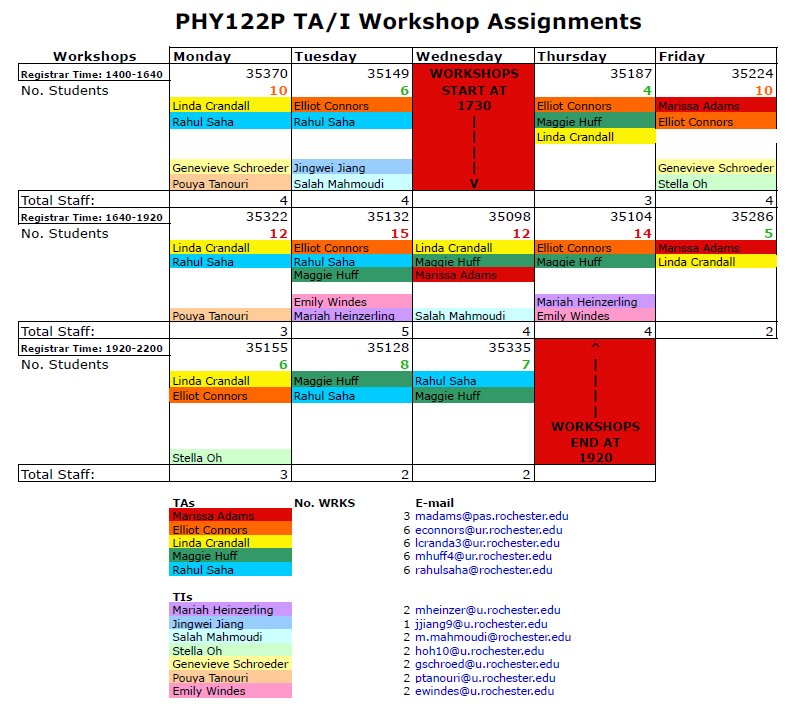
\includegraphics[width=.8\textwidth]{Figures/ExampleWorkshopSchedule.png}
  \caption{\protect\label{fig:egws} The workshop schedule for PHY122P in the Fall of 2016.}
\end{figure}

\indent Finding a balance with the number of staff you are given to work with, and the number of students who typically come to those workshops lends making a workshop schedule to be an iterative process. An example of a workshop schedule is given by Figure \ref{fig:egws}. This was the final iteration of the workshop schedule for that year and was established by the end of September. So open up EXCEL, or LibreOffice, and allow \texttt{COUNTIF} to become your new best friend. Note the following information on the schedule:

\begin{enumerate}
	\item There are generally three workshops per day during the ``work week'' (Note \emph{Registrar Time}). Typically one starts off with 13 workshops, and then may take some away as illustrated. Traditionally we've left off the Friday night workshop.
		\begin{enumerate}
			\item ``Afternoon'' workshops; generally 14:00-16:40 according to the registrar.
			\item ``Evening'' workshops; generally 16:40-19:20 according to the registrar.
			\item ``Night'' workshops; generally 19:20-22:00 according to the registrar.
		\end{enumerate}
	\item Students do not need to stick with the workshop they have registered for. They simply need to be registered for a workshop. However generally they'll register for the one they like the most. This will give you an idea of the attendance for that workshop before the semester begins (Note \emph{No. Students}, the professor can inform you of who and how many students are registered from being designated as ``Instructor'' on the blackboard). This will give you an idea of how many people to schedule for a given workshop.
	\item The workshop registration code is also included for easy access, as sometimes communication about cancelling workshops, and which students need to move, requires the code.
	\item Ensure that the professor for the course cancels the Wednesday afternoon workshop as it conflicts with the department colloquium. Students registered for that workshop can visit the professor for the course or the undergraduate adviser to re-register.
	\item After the first couple of weeks, you can gauge the typical attendance of each workshop by querying the staff at group meetings. Workshops where no students are showing up can also be cancelled.
	\item Workshops with high attendance should have more staff, workshops with low attendance to not require too many people (Note \emph{Total Staff} is tallied at the end of each workshop).
	\item Include the contact information (e-mail) for the staff.
	\item Color coordinating helps the staff get an idea of where they fit into the schedule, and if they like the pattern they see in the context of their life. Color can be really helpful for also distinquishing between TA/Is and how many people need to be in what workshop.
\end{enumerate}

\indent After you've developed your first workshop schedule, and it has been approved by the professor and staff, it is time to go public. Post it to the blackboard, and print out copies to post around the workshop room. Note that wherever you have posted the first workshop schedule, you will need to replace again if you work up an improved one.

%%%%%%%%%%%%%%%%%%%%%%%%%%%%%%%%%%%%%%%%%%%%%%%%%%%%%%%%%%%
\subsection{Blackboard} \label{sec:bb}

As a Teaching Assistant for the course, the professor will have most likely added you to the course website at \url{learn.rochester.edu}, along with the rest of the staff for the course. Once you have logged into the website using your UR NetID and password, you should be able to observe the course listing for the MSP course you're teaching. 

\indent After clicking the link you should be brought to the \emph{Announcements} page. The course web page is accessible to all students. However as a Teaching Assitant you have special privileges to create links hidden from students. All of the links are featured on the left side bar, however hidden links include a box with a line through the diagonal. An example of this is provided in Figure \ref{fig:egannouncement}, note the links with the slashed-box icon. 

\indent Blackboard is a utility that is not just useful for communication with students and delivering documents, but also doing so for the staff (including professors, administrators, workshop and laboratory TA/Is). Adhering to an organized course web-page structure and directory tree can be crucial to the workflow for the students, staff, as well as yourself. The following are guidelines on what to post on the Blackboard, but how you do so is up to you and the professor of the course.

\begin{figure}[h]
  \centering
      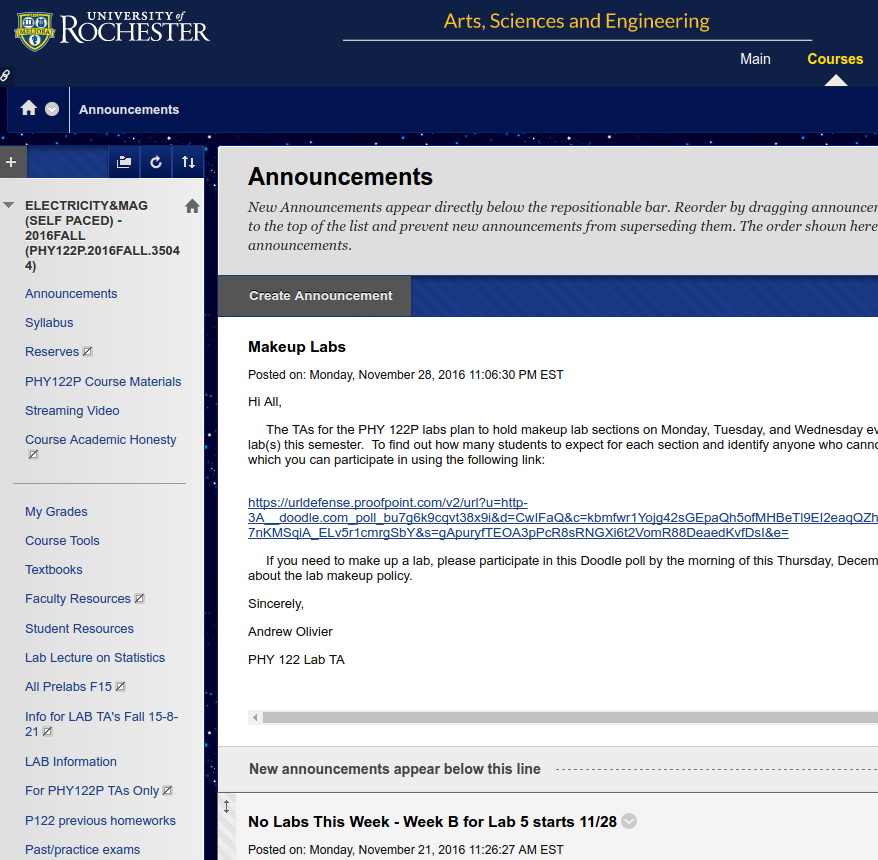
\includegraphics[width=.8\textwidth]{Figures/BBAnnouncements.png}
  \caption{\protect\label{fig:egannouncement} The announcement webpage of PHY122P for Fall 2016.}
\end{figure}

%%%%%%%%%%%%%%%%%%%%%%%%%%%%%%%%%%%%%%%%%%%%%%%%%%%%%%%%%%%
\subsubsection{Adding Materials to Blackboard} \label{sec:bbres}

\indent Note that actually ``creating'' components, announcements and directories on Blackboard is fairly straight forward. On whatever link page you're on you can ``build content'' of your choosing. 

\noindent \textbf{List of materials to be put on blackboard for TAs:} Ensure that a hidden link is created for TA/I material only.

\begin{itemize}
	\item A directory including the PHY122P study guides/workshops with solutions.
	\item If you decide to provide prescreens questions, the prescreens and solutions are included for each module within their own directory.
	\item Giancoli Textbook and Solutions (which can also be an aid for prescreens).
		\begin{itemize}
			\item Make sure you include the following highlight post on the content item: ``\emph{Note: Giancoli, Physics for Scientists and Engineers 4th edition, is copyrighted material and cannot be shared outside of blackboard.}''
		\end{itemize}
	\item The literature provided in the git-repo \ref{sec:gitrepo} on MSP courses.
	\item The literature provided in the git-repo \ref{sec:gitrepo} for TA/I training.
\end{itemize}

\noindent \textbf{List of materials to be put on blackboard for students:} Please note that it is not your duty to provide laboratory materials on blackboard, but that responsibility is for the TAs associated with the laboratory portion of the course.

\begin{figure}[h]
  \centering
      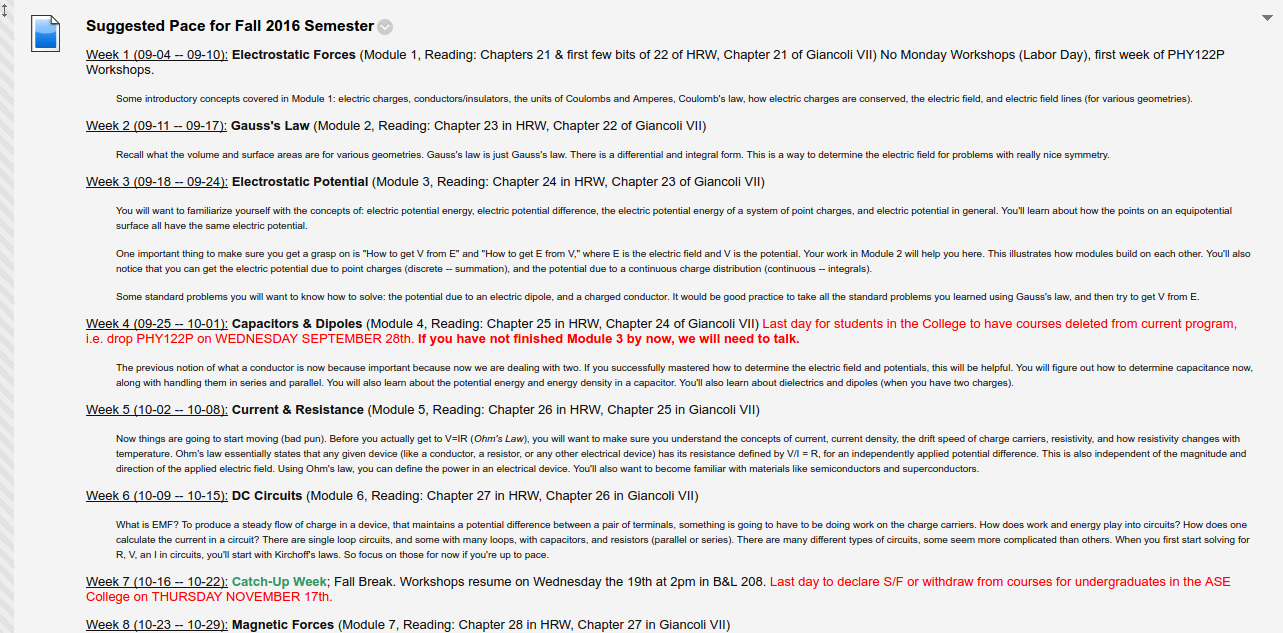
\includegraphics[width=1\textwidth]{Figures/SuggestedPace.png}
  \caption{\protect\label{fig:suggpace} A screenshot of a section of the suggested pace provided to the students on Blackboard for PHY122P Fall 2016.}
\end{figure}

\begin{itemize}
	\item The syllabus: This could be just a written document, or the presentation given by the professor for the initial sole lecture given at the beginning of the semester.
	\item Course Materials
		\begin{itemize}
			\item Make this it's own directory link.
			\item Post all of the module workshops/study guides before the semester begins in their own directory (without solutions).
			\item The document, ``How to Get an A in PHY122P,'' which can be found in the git-repo \ref{sec:gitrepo}.
			\item The suggested pace for the semester
				\begin{itemize}
					\item In tandem with the schedule put out by the university (i.e. note when the semester begins, ends, breaks, and holidays are) construct a suggested pace for a student in the course. Generally the rule of thumb is one module per week. You can see an example of how the suggested pace is typically relayed to students in Figure \ref{fig:suggpace}.
				\end{itemize}
			\item Important schedules
				\begin{itemize}
					\item The current TA/I workshop schedule (each iteration, delete and upload the current copy)
					\item The google spreadsheet for the quiz slot schedule
				\end{itemize}
			\item Previously some courses have offered the PDF version of Giancoli Edition 4 to blackboard
				\begin{itemize}
					\item Make sure you include the following highlight post on the content item: ``\emph{Note: Giancoli, Physics for Scientists and Engineers 4th edition, is copyrighted material and cannot be shared outside of blackboard.}''
				\end{itemize}
		\end{itemize}
	\item The material in the workshops and study guides may not be enough to help students prepare for their module examinations or the final (despite textbooks having a multitude of problems, they may prefer more stuctured things). You may want to post, with professor permission,
		\begin{itemize}
			\item Previous PHY122 (lecture based) homeworks.
			\item Old practice/exams from PHY114 or PHY122.
		\end{itemize}
	\item A note about academic honesty.
\end{itemize}

%%%%%%%%%%%%%%%%%%%%%%%%%%%%%%%%%%%%%%%%%%%%%%%%%%%%%%%%%%%
\subsubsection{Adding Students to Blackboard Course Page} \label{sec:addstuds}

\indent In the beginning of the semester students will be adding and dropping the course. Students who have been added after the online registration deadline may need for you to add them directly to the course through Blackboard. To do this look down the left-column with links under the header, \emph{Course Management}. From there do the following, \textbf{Users and Groups} > \textbf{Users} > \textbf{Find Users to Enroll}. The student has probably contacted you via e-mail. If their e-mail is a rochester e-mail, their username will be the username to search for. Ensure to enroll them as a student.

\indent You can follow the same process for adding Teaching Assistants and Instructors to blackboard, but adding them as TAs.

%%%%%%%%%%%%%%%%%%%%%%%%%%%%%%%%%%%%%%%%%%%%%%%%%%%%%%%%%%%
\subsubsection{E-mails} \label{sec:emails}

To send an e-mail out via blackboard to the class you follow a comparable process to adding a student: \textbf{Course Management} > \textbf{Course Tools} > \textbf{Send Email}. You will then be confronted with a number of options, as Blackboard will state, ``Instructors can send email to all or selected individual Users, Students, Groups, Teaching Assistants, Instructors or Observers. From a Blackboard Learn course, email cannot be sent to anyone who is not a member of the course.'' The course relies heavily upon e-mail.

%%%%%%%%%%%%%%%%%%%%%%%%%%%%%%%%%%%%%%%%%%%%%%%%%%%%%%%%%%%
\subsubsection{Grade Center} \label{sec:gc}

To access the Grade Center follow \textbf{Course Management} > \textbf{Grade Center} > \textbf{Full Grade Center}.

\subsubsubsection{Grade Center Set Up}

\noindent The grade center should have columns in the following order, but read from left to right. Some of the columns with values will be generated automatically by Blackboard. This is the optimal setting for the \emph{progressplot.py} to read the downloaded grade center as:

\begin{itemize}
	\item Last Name
	\item First Name
	\item Student ID
	\item Username
	\item Last Access
	\item Total
	\item N Labs to be dropped
	\item Final exam score
	\item Attendance
	\item Tests Completed
	\item Total Quizzes 1-12
	\item All Postlabs
	\item All Prelabs
	\item The next set of couples effectively follows:
	\begin{mdframed}[style=CommandFrame]
	\texttt{\textbf{for} x \textbf{in} int(NumModules): \\
			\hspace{10pt} \textbf{print} "Module "+x+" Version"+"$\backslash$n"+"Module "+x+" Grade"}
	\end{mdframed}
	The \emph{progressplot.py} will effectively search for a header of the title "Module 1 Version" and then iterate from there.
	\item N or incomplete?
	\item Waiver
	\item Similarly to the modules and their grades, we have the labs:
	\begin{mdframed}[style=CommandFrame]
	\texttt{\textbf{for} x \textbf{in} int(NumLabs): \\
			\hspace{10pt} \textbf{print} "Prelab"+x+$\backslash$n"+"PostLab"+x}
	\end{mdframed}
	\item Quizzes Passed
	\item Quiz Grade
	\item Lab Grade
	\item Average
	\item Letter Grade
\end{itemize}

\subsubsubsection{Grade Center Download} \label{sec:gradecenterdownload}

\noindent To download the Grade Center, follow: \textbf{Course Management} > \textbf{Grade Center} > \textbf{Full Grade Center} > \textbf{Work Offline} > \textbf{Download}. Select \textbf{Full Grade Center}, with delimiter type of \textbf{Comma}, and included hidden information type \textbf{No}. You can choose where to save the location. Then hit submit. Never upload a new grade center, or download while the workshops are in session, or whenever you can expet blackboard to be used heavily for a period of time by TA/Is.

\subsubsubsection{Tracking Changes} \label{sec:trackchanges}

\noindent Note that one can track the changes made in the Grade Center. This can be really important if you want to check the pass rates of the TA/Is who are grading, see \ref{sec:ft}. To do this: \textbf{Course Management} > \textbf{Grade Center} > \textbf{Full Grade Center} > \textbf{Reports} > \textbf{View Grade History} > \textbf{Download}. You can then choose download options as you would to download the full grade center spreadsheet.

%%%%%%%%%%%%%%%%%%%%%%%%%%%%%%%%%%%%%%%%%%%%%%%%%%%%%%%%%%%
\subsection{Quiz Schedule} \label{sec:qs}

\indent The quiz schedule is a crucial component to the organization and movement of the MSP class. Find an spreadsheet application that is accessible to the public (particle the PHY12$X$P community) to view, and for those managing the course to edit. The historically used application is \emph{Google Docs}. If a new, better suited, application comes into development, test it out. The Fall 2016 PHY122P Module Quiz Schedule is still online at \url{https://docs.google.com/spreadsheets/d/12zjeavARTm9qDs9g9xELc7jxhnrU73wDJzVnRHM830s}. The reader is welcome and encouraged to copy and paste the format of this document for future usage.

\indent The purpose of the quiz schedule is so that students can see the availability of quiz slots so that they can schedule and take their quiz (as the name states). A number of factors go into making the quiz schedule, in particular, the number of quiz slots and when they are:

\begin{itemize}
	\item The University Calendar: when classes begin and end, holidays, and breaks.
	\item The TA/I schedule, see \ref{sec:schedule}, i.e. the number of workshops in combination with the number of graders in the workshop.
	\item The number of students registered in the course (students should pass modules at a rate of 1.8-2 attempts/module).
\end{itemize}

\indent The general form of the quiz schedule involves a variety of sheets. You should have a sheet for each week in the semester. The title of the sheet should be the beginning day of the week. It is best to get this document completed before the semester begins. On that week's sheet you should have the following information:

\begin{itemize}
	\item Two columns per day.
	\item For the headers for each day:
		\begin{itemize}
			\item \textbf{Row 1:} The first column has the title, \textbf{Date: (e.g. Monday)}, while the second column has the date for that day, \textbf{09/5/16}. One can utilize the calendar capabilities of Google Docs, and easily copy and page for each week.
			\item \textbf{Row 2:} Column 1, \textbf{Available Slots}, Column 2, is a \texttt{COUNTIF} statement for the number of slots below, e.g. \texttt{=countif(C5:C1000,"<>")-countif(D5:D1000,"<>")}.
			\item \textbf{Row 3:} Column 1, \textbf{Available Slots [\%]}, Column 2, \texttt{=D2/COUNTIF(C5:C1000,"<>")}, which calculates the average for the Row 2 values.
			\item \textbf{Row 4:} Next we have the headers for the slots; Column 1, \textbf{Time}, Column 2, \textbf{Student ID}.
		\end{itemize}
	\item Based on your quiz slot rate calculation, you can then list the times for the quiz slots in Column 1.
	\item In Column 2, students will put their ID numbers.
	\item Iterate this process for all of the days there are workshops.
	\item Once that is done, make another two-column set. For Rows 1-3, have it count up the number of unused quiz slots (sum, all of the available quiz slots), the number of given slots for that week (the ratio of say, \texttt{D2/D3}, and then the percentage of how many went unused.
\end{itemize}

\indent There is one special sheet that can be incredibly useful: the quiz slots statistics. At the front of all the other weekly sheets, make one that is effectively a summary. Pull the information off of the last set of columns visualize them on this sheet in a readable way. From there you can calculate how many slots are available, were wasted, and quizzes taken as the semester goes on. Using the number of students, slots left, average number of modules off of the progress plot history/remaining number of modules, you can figure out how many exams per student are left.

\indent Once your quiz slots schedule is ready to be used make sure you do the following:

\begin{itemize}
	\item All Teaching Assistants and Instructors have been granted editing their permission. They will need a gmail address.
	\item No easily identifiable student information should be on the sheet. In the past people have used students' names to fill in for the quiz slot. Currently we do this using student ID numbers.
	\item In the workshop room, graders will ask students to ID themselves by their student ID number.
	\item If a student comes on time to their exam, their cell is marked as green. If they come late, their cell is marked red.
	\item Look for student's cells that are marked red and send them an email encouraging them to come to the slots they have signed up for, as they are not a resource to be wasted. They are effectively taking away someone else's potential quiz slot if they do not show up.	
\end{itemize}

%%%%%%%%%%%%%%%%%%%%%%%%%%%%%%%%%%%%%%%%%%%%%%%%%%%%%%%%%%%
\subsection{Observing Course Progress (\texttt{\emph{progressplot.py}})} \label{sec:ocp}

\indent Charting the course progress weekly during the semester is of crucial importance. It allows for not only you, the staff, and the professor to understand how the class is doing, but also allows for an individual student to figure out where they are situated within the course's student body. Charting the course progress also allows for you to target the students who are behind, and work quickly to catch them up to speed. 

\begin{figure}[h]
  \centering
      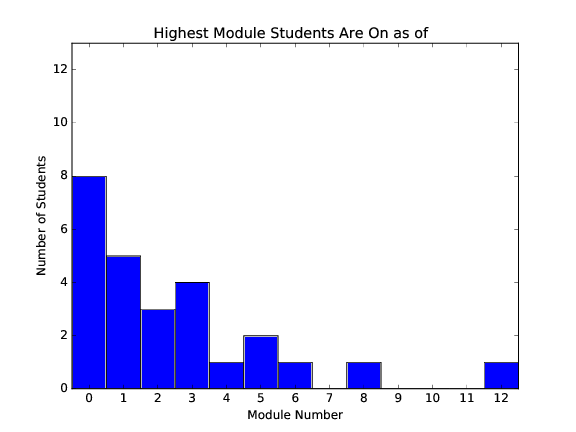
\includegraphics[width=.8\textwidth]{Figures/PHY122P-ProgressPlot.png}
  \caption{\protect\label{fig:progplot} A progress plot using pseudo-student information. Normally the title would include the date for which the grade center was downloaded, however we have scrapped the date from an example grade center.}
\end{figure}

\indent A helpful tool we use to chart the course progress is a python script, called \emph{progressplot.py}. One can find this script in the git-repo, \ref{sec:gitrepo} under \emph{ProgressPlot/}. When run, it produces a histogram, comparable to the one shown in Figure \ref{fig:progplot}. However this isn't the only information that the \emph{progressplot.py} can yield. When you run the script in the command line, it pipe's the output to the terminal window, e.g.

\begin{mdframed}[style=CommandFrame]
\texttt{python progressplot.py gc\_PHY12XP.2000FALL.35044\_ \\ fullgc\_2000-01-01-01-01-01.csv 0 22 24}
\end{mdframed}

\noindent which is the command you would run on the grade center comma separated value file you've downloaded from blackboard. You can find the instructions to download the grade center in \ref{sec:gradecenterdownload}. In essence this command is saying, ``Hey python, can you run this script I wrote for you using this file called, \emph{gc\_PHY12XP.2000FALL.35044\_fullgc\_2000-01-01-01-01-01.csv} and then give me some information for Module Number 0, student contact, and module signifier information which are located in columns 22 to 24 in said file?''

\indent The output of this command:

\begin{mdframed}[style=CommandFrame]
(1) > ['F', 'F', '6', 'F@u.rochester.edu'] ['', ''] \\
(2) > ['G', 'G', '7', 'G@u.rochester.edu'] ['', ''] \\
(3) > ['H', 'H', '8', 'H@u.rochester.edu'] ['', ''] \\
(4) > ['K', 'K', '11', 'K@u.rochester.edu'] ['', ''] \\
(5) > ['O', 'O', '15', 'O@u.rochester.edu'] ['', ''] \\
(6) > ['Q', 'Q', '17', 'Q@u.rochester.edu'] ['', ''] \\
(7) > ['R', 'R', '18', 'R@u.rochester.edu'] ['', ''] \\
(8) > ['S', 'S', '19', 'S@u.rochester.edu'] ['', ''] \\
(9) > TOTAL \# OF STUDENTS:  26 \\
(10) > VALUES ON HISTOGRAM \\
(11) > ( Module \#, \# of Students Passed ) \\
(12) > ( 0 , 8 ) \\
(13) > ( 1 , 5 ) \\
(14) > ( 2 , 3 ) \\
(15) > ( 3 , 4 ) \\
(16) > ( 4 , 1 ) \\
(17) > ( 5 , 2 ) \\
(18) > ( 6 , 1 ) \\
(19) > ( 7 , 0 ) \\
(20) > ( 8 , 1 ) \\
(21) > ( 9 , 0 ) \\
(22) > ( 10 , 0 ) \\
(23) > ( 11 , 0 ) \\
(24) > ( 12 , 1 ) \\
(25) > Average Module:  2.42307692308 \\
(26) > Median:  1.5 \\
(27) > Standard Deviation:  2.84433413761
\end{mdframed}

\indent The grade center used for this is a test version that utilizes pseudo-student data. Again, you can find it in the git-repo, \ref{sec:gitrepo}. The same information is reflected in Figure \ref{fig:progplot}. The above lines can be deciphered like so:

\begin{itemize}
	\item Lines (1)--(8) are the student contact inform for the columns queried (i.e. 22 to 24 (not inclusive -- so really 22 and 23)), along with their module signifier. These pseudo-students apparently have no module signifier because they are the eight students on module zero and have not started, or even prescreened for module one.
	\item Line (9) tells you the number of students enrolled in blackboard.
	\item Lines (11)--(24) tell you the hard numbers illustrated by Figure \ref{fig:progplot}.
	\item Lines (25)--(27) tell you the statistics of the histogram.
\end{itemize}

\noindent So what does one do with the progress plot and all of the associated information?

\begin{itemize}
	\item Make sure if you're using a new grade center, that you download it from the Blackboard at a time when other TAs and TIs will not be accessing it (so before or after the workshops are over).
	\item You may want to run this script once, or perhaps more times each week.
	\begin{itemize}
		\item Send a weekly e-mail to students with the suggested pace, and the current status of the course (via the progress plot) to determine how well the class is following the suggested pace. In this e-mail you can also include a bunch of other added information (resources for the suggested pace module, the module students are stuck on, etc). \textbf{Do not send student specific information out to the class, only general numbers about the class as a whole (historgram, mean, median, mode, standard deviation, etc).}
		\item You will also want to send an e-mail to Nick Valentino (\ref{sec:ppl}) perhaps once or twice a week. This e-mail should include the information you've sent the students, but also the specific students that are behind. From there he will contact those students and help provide solutions and support for them.
	\end{itemize}
	\item At the end of the class you can make a nice gif of all the progress plots (you'll want to normalize the y-axis, or number of students).
\end{itemize}

%%%%%%%%%%%%%%%%%%%%%%%%%%%%%%%%%%%%%%%%%%%%%%%%%%%%%%%%%%%
\subsection{Checking Pass Rates} \label{sec:cpr}

\noindent The pass rate refers to the rate at which $X_{i}$ is passed per exam. Here $X_{i} = \{$ module quizzes given for the class, module quizzes given by a particular TA $\}$. These items in $X_{i}$ should correspond one-to-one. In this section we go over how to check both of these items. Pass rates are important to check occasionally as they indicate the status of a module or grader (are we giving out too many of the same quizzes? is one module particularly easier then an other? is Jeremy too easy of a grader?), which can allow you to delegate attention and help to a particular part of a course. This is generally information that is not disseminated to the student body, but is rather shared among the staff and professor.


%%%%%%%%%%%%%%%%%%%%%%%%%%%%%%%%%%%%%%%%%%%%%%%%%%%%%%%%%%%
\subsubsection{For Students (\texttt{\emph{passrate.py}})} \label{sec:fs}

\noindent To check the pass rate for each module quiz among the student body we consider the following questions:

\begin{enumerate}
	\item What is the total number of quizzes given to the student body?
	\item What is the number of quizzes given for each module?
	\item Thus, what is the percentage of module quizzes given for a particular module?
	\item What is the total number of prescreens given to the student body?
	\item What is the number of prescreens given for each module?
	\item What is the ratio between the number of quizzes given per number of prescreens given?
\end{enumerate}

\noindent All of these questions are addressed by a script called \emph{passrate.py}, which can be found in the git-repo (\ref{sec:gitrepo}) via the path \directory{PHY12XP\_HeadTAMaterials/ProgressPlot}. Using the example grade center in the same directory we are given the following output after the command,

\begin{mdframed}[style=CommandFrame]
\texttt{python passrate.py gc\_PHY12XP.2000FALL.35044\_ \\ fullgc\_2000-01-01-01-01-01.csv}
\end{mdframed}

\noindent The output of this command:

\begin{mdframed}[style=CommandFrame]
(1) > Number of Quizzes Given Each Module: [1, 2, 3, 4, 5, 6, 7, 8, 9, 10, 11, 12] =  [27, 21, 20, 7, 6, 3, 4, 5, 2, 1, 1, 1] \\
(2) > Total Number of Quizzes Given According to Blackboard:  98 \\
(3) > \% of Module 1 Quizzes:  27.5510204082 \\
(4) > \% of Module 2 Quizzes:  21.4285714286 \\
(5) > \% of Module 3 Quizzes:  20.4081632653 \\
(6) > \% of Module 4 Quizzes:  7.14285714286 \\
(7) > \% of Module 5 Quizzes:  6.12244897959 \\
(8) > \% of Module 6 Quizzes:  3.0612244898 \\
(9) > \% of Module 7 Quizzes:  4.08163265306 \\
(10) > \% of Module 8 Quizzes:  5.10204081633 \\
(11) > \% of Module 9 Quizzes:  2.04081632653 \\
(12) > \% of Module 10 Quizzes:  1.02040816327 \\
(13) > \% of Module 11 Quizzes:  1.02040816327 \\
(14) > \% of Module 12 Quizzes:  1.02040816327 \\
(15) > Total number of Prescreens per Module:  [1, 2, 3, 4, 5, 6, 7, 8, 9, 10, 11, 12] =  [23, 14, 10, 10, 6, 3, 3, 2, 1, 1, 1, 1] \\
(16) > Total Number of Prescreens:  75 \\
(17) > Module 1: Number of Quizzes Given/Number of Prescreens Given:  1.17391304348 \\
(18) > Module 2: Number of Quizzes Given/Number of Prescreens Given:  1.5 \\
(19) > Module 3: Number of Quizzes Given/Number of Prescreens Given:  2.0 \\
(20) > Module 4: Number of Quizzes Given/Number of Prescreens Given:  0.7 \\
(21) > Module 5: Number of Quizzes Given/Number of Prescreens Given:  1.0 \\
(22) > Module 6: Number of Quizzes Given/Number of Prescreens Given:  1.0 \\
(23) > Module 7: Number of Quizzes Given/Number of Prescreens Given:  1.33333333333 \\
(24) > Module 8: Number of Quizzes Given/Number of Prescreens Given:  2.5 \\
(25) > Module 9: Number of Quizzes Given/Number of Prescreens Given:  2.0 \\
(26) > Module 10: Number of Quizzes Given/Number of Prescreens Given:  1.0 \\
(27) > Module 11: Number of Quizzes Given/Number of Prescreens Given:  1.0 \\
(28) > Module 12: Number of Quizzes Given/Number of Prescreens Given:  1.0 \\
\end{mdframed}


\indent Lines (1)--(14) effectively give you the same information that one can find on the histogram via \emph{progressplot.py}. If you know how many quizzes you have printed, this can be useful information. You can also alter the script to see how many quizzes are given of a certain type, e.g. Quiz A, B or D for module 5 are given more often than Quiz C, so you can instruct the graders to hand out more of Quiz C. Lines (15)--(28) inform you of how well the contingencies (prescreens) are, or give you're giving enough prescreens for a particular module. You can see from this output that modules 3, 8, 9 need to have an increase in prescreens; too many quizzes are being given without prescreen. Depending on how you have set up the prescreen rules (say only prescreen for the first try, and again if one has failed after the second try, you may then want to have students prescreen for every try on that module, or make students work harder at that module's prescreen). It could also be a matter of staff forgetting to input an ``R'' in blackboard module value column for ``ready for quizzing,'' i.e. the student has passed a prescreen. 

\indent Effectively this script gives you an idea of how to apply emphasis to problem areas in the course.


%%%%%%%%%%%%%%%%%%%%%%%%%%%%%%%%%%%%%%%%%%%%%%%%%%%%%%%%%%%
\subsubsection{For TA/Is} \label{sec:ft}

\noindent One can also query for the pass rates of each of the individual graders who have been inputting grades (pass or fail) into blackboard. This is important as the graders should aim to keep a pass rate of 60\%. If someone is too harsh and way below this value, or too easy, you and the professor will want to talk to them about how they grade, and perhaps shadow them during the workshop and give feedback.

\indent To access the changes made to blackboard's grade center, recall in \ref{sec:trackchanges} how one can download a comma separated value file. After doing this, you can import the file into your favorite spreadsheet editor, and then search for useless information to delete. Effectively you will want to whittle down the spreadsheet until you have the graders' input information left over. You'll want to \texttt{COUNTIF} the following information:

\begin{itemize}
	\item On average: the total number of quizzes graded, the total number passed, the total number failed, and thus the pass rate.
	\item You can then replicate this process for each of the individual TA graders.
\end{itemize}

%%%%%%%%%%%%%%%%%%%%%%%%%%%%%%%%%%%%%%%%%%%%%%%%%%%%%%%%%%%
%%%% RESOURCES %%%%%%%%%%%%%%%%%%%%%%%%%%%%%%%%%%%%%%%%%%%%
%%%%%%%%%%%%%%%%%%%%%%%%%%%%%%%%%%%%%%%%%%%%%%%%%%%%%%%%%%%
\section{Resources} \label{sec:resources}
%%%%%%%%%%%%%%%%%%%%%%%%%%%%%%%%%%%%%%%%%%%%%%%%%%%%%%%%%%%

%%%%%%%%%%%%%%%%%%%%%%%%%%%%%%%%%%%%%%%%%%%%%%%%%%%%%%%%%%%
\subsection{git Repository} \label{sec:gitrepo}

\indent There exists a \texttt{git} repository that includes the materials described throughout this document at \url{https://github.com/madams15/PHY12XP\_HeadTAMaterials}. The repository, or ``repo,'' also includes the working directory for this document. The purpose of having a repo for this course is to have all of the necessary tools at hand for future Head/Teaching Assistants/Instructors, Professors, and potentially Instructors for even the summer sessions. No one wants to reinvent the wheel, however if there are new tools that one wants to develop they are welcome to contribute to the repo (\ref{sec:contributions}) and give themselves authorship over their development. However ensure that you supply an adequate amount of documentation and commentary about the new tool. The bare minimum asked is a brief description of it's purpose, and location in the directory tree, in the \emph{README.md}. You can see an example of the \emph{README.md} in \ref{sec:readme}.

\indent The suggested usage, or workflow, for using the \texttt{git} repo would be to download it (\ref{sec:downloadrepo}), and then create a separate, and parallel working directory outside of the repo for yourself. Copy the tools and documents needed from the repo to your own directory. As the semester goes on your personal directory will become populated with progress plots, and grade centers from blackboard, for example. This is confidential student information you will want to keep separate from materials that you may accidentally \texttt{push} into the repository. If you develop a tool, wait till the end of the semester once you've honed it, and documented it, and then move it to your downloaded repo, and \texttt{push} it in. We aim to keep the materials in the repo as general as possible for future iterations of the course.

%%%%%%%%%%%%%%%%%%%%%%%%%%%%%%%%%%%%%%%%%%%%%%%%%%%%%%%%%%%
\subsubsection{Directions for Download} \label{sec:downloadrepo}

Here are some instructions for downloading, or \texttt{clone}-ing the repository. This may be beneficial to those who have never used \texttt{git} before or worked in the command line. You can also simply google for ``how to use \texttt{git},'' but here we specifically go through the steps using the pertinent links. If you have used \texttt{git} before, feel free to completely ignore this section. If you have no desire to learn, and just want to grab all the goodies, you can easily download the repository in the browser of your choosing by following the link provided in \ref{sec:gitrepo}.

\begin{enumerate}

\item \textbf{Operating System: }To begin first ask yourself what operating system you're working on. If you're working in Linux or Mac (UNIX-based) you'll be okay. However if you're working with Windows, I cannot help you.

\item \textbf{Text Editors:} In order to use the scripts you may need to do a minor bit of coding. Explore some text editors that you feel most comfortable with. The best one to use is \texttt{emacs}. One can simply open up a document by typing

\begin{mdframed}[style=CommandFrame]
\texttt{emacs python\_script.py -nw}
\end{mdframed}

and then saving and closing by holding down CRTL-x, CRTL-s, then CRTL-x CRTL-c.

\item \textbf{Basic UNIX Commands:} Open up your terminal application, and then type

\begin{mdframed}[style=CommandFrame]
\texttt{cd $\sim$/Documents/}
\end{mdframed}

\noindent and press enter. You can \texttt{cd} into whatever directory you would like to download the repo into (note that \texttt{$\sim$/} represents your ``home'' directory). To check where you are in the terminal, you can use the command

\begin{mdframed}[style=CommandFrame]
\texttt{pwd}\\
> \emph{/home/Documents/}
\end{mdframed}

\noindent which will return your path. If you want to see what is in the directory you currently reside,

\begin{mdframed}[style=CommandFrame]
\texttt{ls} \\
> \emph{passrate.py}
\end{mdframed}

\noindent to see the contents (e.g. the contents of this directory is \emph{passrate.py}). If you want to move ``up'' and ``down'' within your directory tree, you can keep using \texttt{cd} with the appropriate path. To move back a directory, or however many, you can do like so:

\begin{mdframed}[style=CommandFrame]
\texttt{cd ../ \\
 cd ../../}
\end{mdframed}

\noindent ``\texttt{../} represents moving back one directory, where as ``\texttt{../../}'' represents moving back two. One can repeat this process for however many directories they know they need to move back by. Also note that the current directory in which one resides is represented by one dot, i.e. ``\texttt{./}.'' 

To copy something one can use the command \texttt{cp <file>}. To copy a bunch of files, or files that are recursively within a directory tree, \texttt{cp -rf <files \& path>}. To remove files the command is \texttt{rm} (use with caution). To move files, the command is \texttt{mv}. The recursive ``force'' (\texttt{-rf}) applies to these commands as well. If you ever want to learn more about a command in general, you can type \texttt{man <command>} in the command line and see the manual page for that command. To page down you hit CTRL-v, and to exit simply press ``q'' for quit.

These are some basic UNIX commands to use in the command line of your terminal application. Getting quick and comfortable with them takes time and patience.

\item \textbf{Downloading using \texttt{git}: } Simply copy and paste the following command into the command line in the directory you wish the repository to be
\begin{mdframed}[style=CommandFrame]
\texttt{ git clone \\ \url{https://github.com/madams15/PHY12XP\_HeadTAMaterials.git}}
\end{mdframed}

\noindent Then go into the project to work in it, or \texttt{cp} things out of it

\begin{mdframed}[style=CommandFrame]
\texttt{cd PHY12XP\_HeadTAMaterials/}
\end{mdframed}

\end{enumerate}

%%%%%%%%%%%%%%%%%%%%%%%%%%%%%%%%%%%%%%%%%%%%%%%%%%%%%%%%%%%
\subsubsection{Contributing to the Repo} \label{sec:contributions}

Say you have developed a new script (\emph{new\_script.py}) that does some fancy statistics on the course progress and you would like to put it in the repo.

\begin{mdframed}[style=CommandFrame]
\texttt{git add new\_script.py}
\end{mdframed}

\noindent or if you want to add everything,

\begin{mdframed}[style=CommandFrame]
\texttt{git add *}
\end{mdframed}

\noindent To then commit these changes or additions,

\begin{mdframed}[style=CommandFrame]
\texttt{git commit -m "My commit message new script"}
\end{mdframed}

\noindent The files are then committed to the HEAD of the local working copy but are not in the remote repository yet. To send these changes to the remote repository, execute

\begin{mdframed}[style=CommandFrame]
\texttt{git push origin master}
\end{mdframed}

\noindent to push to the master branch of the repository.

%%%%%%%%%%%%%%%%%%%%%%%%%%%%%%%%%%%%%%%%%%%%%%%%%%%%%%%%%%%
\subsubsection{README.md} \label{sec:readme}

This is primarily included here in the case that you aren't informed of the repo before reading this document, that you can see what is included and feel encouraged to use it.

\begin{mdframed}[style=MyFrame]

\Large Welcome to \textbf{PHY12$X$P\_HeadTAMaterials}!

\hspace{10pt}

\noindent \textbf{Purpose:} \\
\small
\noindent The purpose of this git repo should be obvious if you have been directed here and you are familiar with the Mastery-Self Paced (MSP) Physics courses taught at the University of Rochester. You are most likely assigned as the role of being the Head Teaching Assistant for the course. Hopefully you find the following set of directories helpful as they should cover all of the materials and instructions  you need for:

\begin{enumerate}
	\item What the course is all about
	\item Managing and training your fellow team of Teaching Assistants and Instructors
	\item Determining the course pace
	\item What action you need to take based on the current course pace and situation in real time
\end{enumerate}

\Large
\noindent \textbf{Table of Contents:}

\small
\noindent Here is the ``Table of Contents'' for this git-repo, including a brief description of each directory, and files of importance. 

\begin{enumerate}
	\item \directory{PHY12XP\_HeadTAMaterials} \\
		Home Directory
	\item \directory{PHY12XP\_HeadTAMaterials/HeadTAInstructions} \\
		Directory containing a LaTeX document that details instructions for the user.
	\item \directory{PHY12XP\_HeadTAMaterials/Literature} \\
		Directory containing literature pertaining to the course. \\
		Information provided by the current chair of the Department, Professor Dan Watson (\url{dmw@pas.rochester.edu}).
	\item \directory{PHY12XP\_HeadTAMaterials/ProgressPlot} \\
		Directory containing an the code to track progress in the course. Also includes an example grade center output from blackboard.
	\begin{enumerate}
		\item \emph{gc\_PHY12XP.2000FALL.35044\_fullgc\_2000-01-01-01-01-01.csv} \\
			An example of the Grade Center downloaded from Blackboard with pseudo-student information.
		\item \emph{passrate.py} \\
			A python script that indicates the passrate for each module, including the ratios of number of quizzes given for each module compared to the number of prescreens given.
		\item \emph{PHY122P-ProgressPlot-.pdf} \\
			An example of the output from the following:
		\item \emph{progressplot.py} \\
			A python script that yields a histogram for the current student progress in the class. It also yields student information off of blackboard for whatever module you choose. It also provides the average module number, median, and standard deviation for the course progress.
	\end{enumerate}
	\item \emph{PHY12XP\_HeadTAMaterials/README.md} \\
		This file.
	\item \directory{PHY12XP\_HeadTAMaterials/StudentMaterials}
	\begin{enumerate}
		\item \directory{PHY12XP\_HeadTAMaterials/StudentMaterials/HTGAA\_forStudents/} \\
			An example document that is helpful for students and makes expectations clear. This directory contains the version for PHY122P. However it can be adapted to PHY121P.
		 \item \directory{PHY12XP\_HeadTAMaterials/StudentMaterials/Prescreens} \\
			An example of a prescreen. Please contact the author for prescreens made for PHY122P. If you would like to make more prescreens, please see the document in \directory{/HeadTAInstructions/} for details on how to make them.
	\end{enumerate}
	\item \directory{PHY12XP\_HeadTAMaterials/TAManagement}
	\item \directory{PHY12XP\_HeadTAMaterials/TATrainingMaterials}
	\begin{enumerate}
		\item \emph{PHY12XP\_HeadTAMaterials/TATrainingMaterials/ \newline Detailed-Instructions-for-Instructors\_PHY122P-F15.pdf} \\
			A document crafted by Arie Bodek, Dev Ashish Khaitan, and Marissa Adams. 
		\item \directory{PHY12XP\_HeadTAMaterials/TATrainingMaterials/Grader}
		\item \directory{PHY12XP\_HeadTAMaterials/TATrainingMaterials/Prescreener}
		\item \directory{PHY12XP\_HeadTAMaterials/TATrainingMaterials/WorkshopLeader} \\
			Each of these directories contain respective LaTeX documents that describe the role a Teaching Assitant, or Teaching Instructor, may play in the workshop, or MSP setting.
	\end{enumerate}
\end{enumerate}

\Large
\noindent \textbf{Download Instructions:}

\small
\begin{enumerate} 
	\item Go to: \url{https://github.com/madams15/PHY12XP_HeadTAMaterials}
	\item Either download directly, or type\\

	\begin{mdframed}[style=CommandFrame]
	
		\footnotesize
		\texttt{ git clone \\ \url{https://github.com/madams15/PHY12XP\_HeadTAMaterials.git}}
		\small
		
	\end{mdframed}
		
in the command line. The repository will then be cloned to your machine. Learn more on working with git here: \\
\url{http://rogerdudler.github.io/git-guide/}.
\end{enumerate}

\Large
\noindent \textbf{Author Information:} \\
\small
Marissa B. Adams \\
Graduate Student \\
Affiliation: University of Rochester, Department of Physics \& Astronomy \\
Office: Bausch \& Lomb Hall 108 \\
E-mail: \url{madams@pas.rochester.edu} \\


\Large
\noindent \textbf{Contributors to the Course:} \\
\small
Dan Watson, Gourab Ghoshal, Arie Bodek, Steve Manly. Contributors to the MSP course development, and future Head TAs, are welcome to add authorship to any documents here they feel need amelioration, and have changed themselves. New tools and commits are always welcome. Please add thorough documentation, and edit the \emph{README.md} to reflect changes.
\end{mdframed}

%%%%%%%%%%%%%%%%%%%%%%%%%%%%%%%%%%%%%%%%%%%%%%%%%%%%%%%%%%%
\subsection{People \& Quick Links} \label{sec:ppl}

\begin{itemize}
	\item General thoughts and concerns about MPS courses should be Dan Watson (\url{dmw@pas.rochester.edu})
	\item Regarding staff numbers and TA/I assignments (say you need more TA/Is), Stephen Teitel assigns positions (\url{stte@pas.rochester.edu})
	\item Regarding the needs of graduate students (Teaching Assistants), reach out to the Graduate Program Coordinator, Laura Blumkin (\url{laura.blumkin@rochester.edu})
	\item Regarding the needs of undergraduate students (Teaching Instructors), reach out to the Undergraduate Coordinator, Lindy Cassidy (\url{lcassidy@pas.rochester.edu})
	\item If you ever end up concerned about a student in the course, or a fellow TA/I, you're encouraged to submit a CARE report: \url{https://www.rochester.edu/care/}
	\item If you want to buy supplies for the classroom or things for the course in general, ask the main office assistant, Cynthia Spencer (\url{cspencer@pas.rochester.edu})
	\item Regarding library information, such as Society of Physics Students (SPS) tutoring in the Physics-Optics-Astronomy (POA) Library, contact Jeff Jones, the POA Library Section Supervisor (\url{jjones@library.rochester.edu})
	\item It is necessary to maintain close contact with the Hajim School of Engineering about the current status of the students who are struggling. You will want to inform
		\begin{itemize}
			\item Nicholas Valentino (\url{nicholas.valentino@rochester.edu}) about the status of students who are behind almost weekly via e-mail. Once you have done this, the Hajim School will help provide addition resources for these students and figure out why they are struggling.
			\item The complete list of faculty advisers is listed here: \url{http://www.hajim.rochester.edu/academics/undergraduate/stemgems/stem\_faculty_advisors.html}
		\end{itemize}
	\item The general academic calendar for The University is at \url{https://www.rochester.edu/registrar/calendar.php}
\end{itemize}


\end{document}